\section{Layout}

\begin{figure}[!htb]
	\minipage{0.48\textwidth}
		\centering
		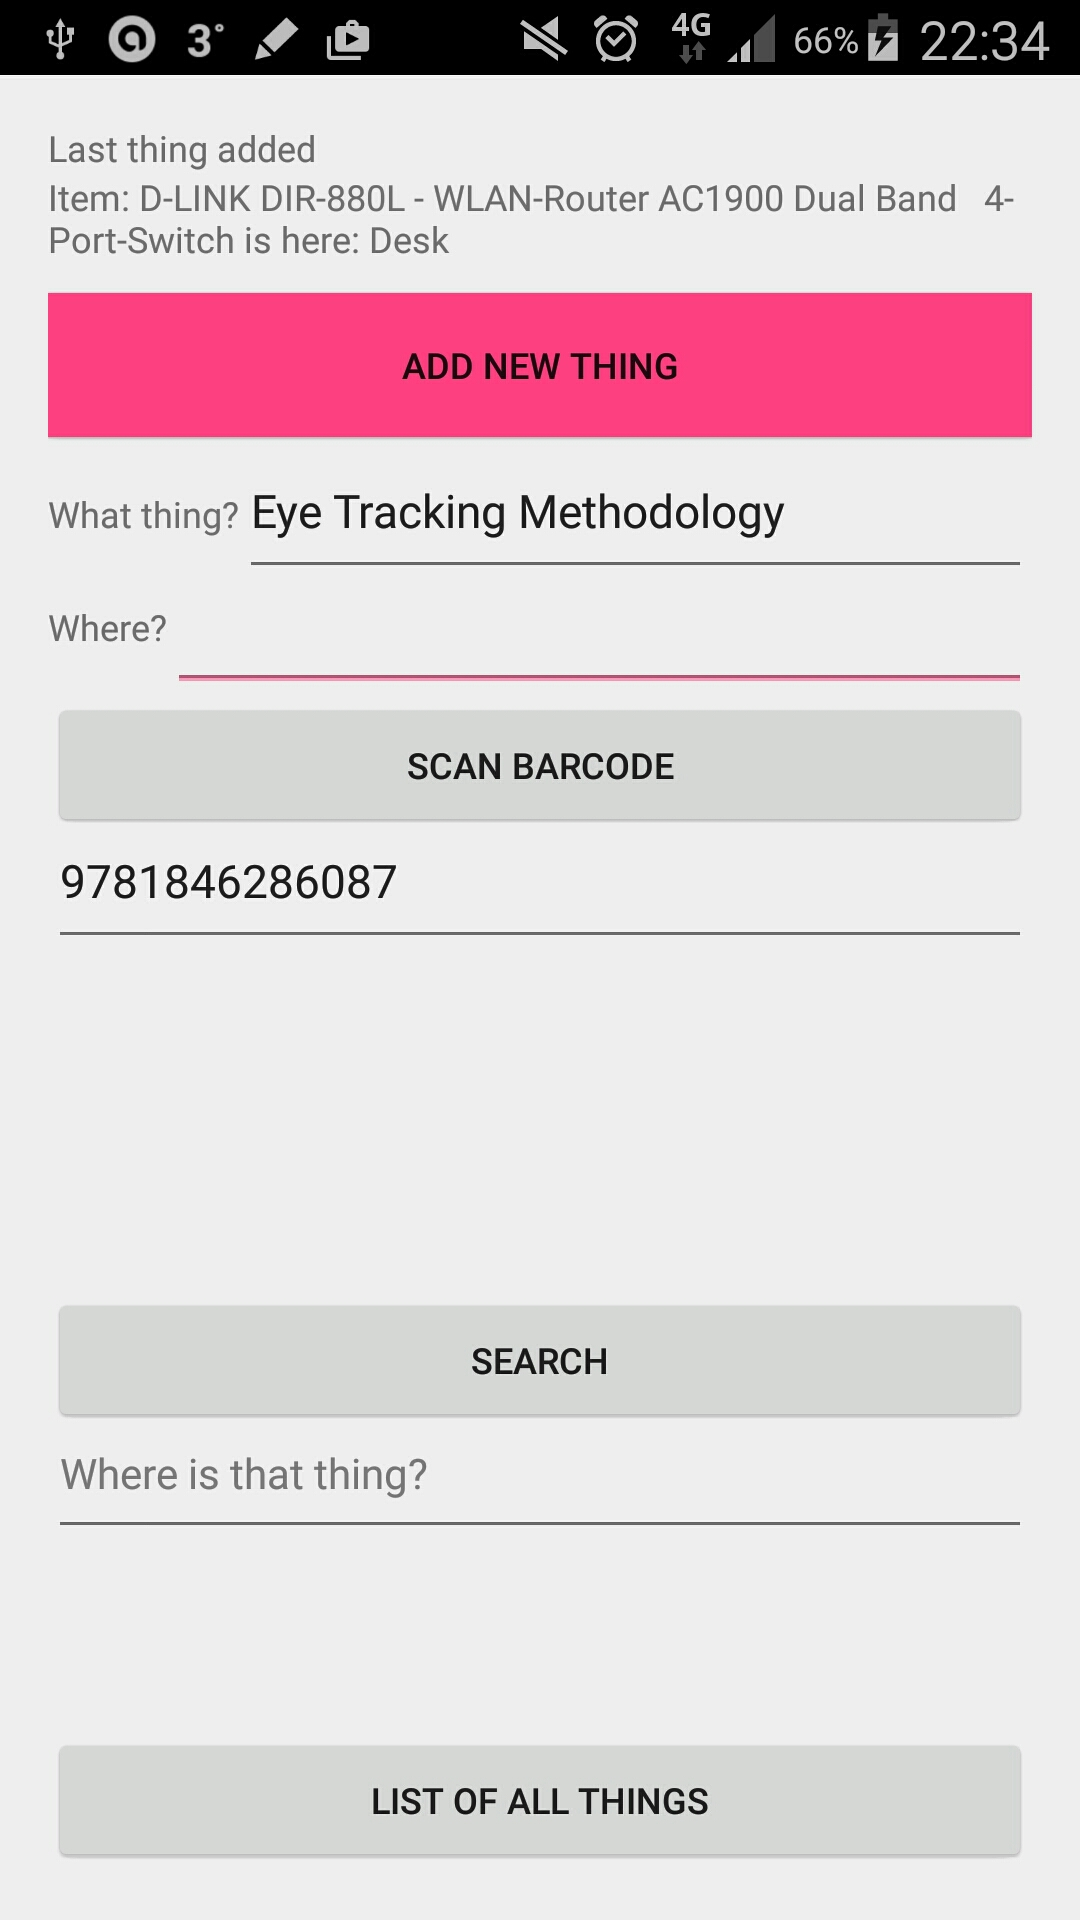
\includegraphics[width=0.9\linewidth]{Tingle-Portrait.jpg}
		\caption{Portrait view of the Tingle Activity.}
		\label{fig:tingle-view-portrait}
	\endminipage\hfill
	\minipage{0.48\textwidth}
		\centering
		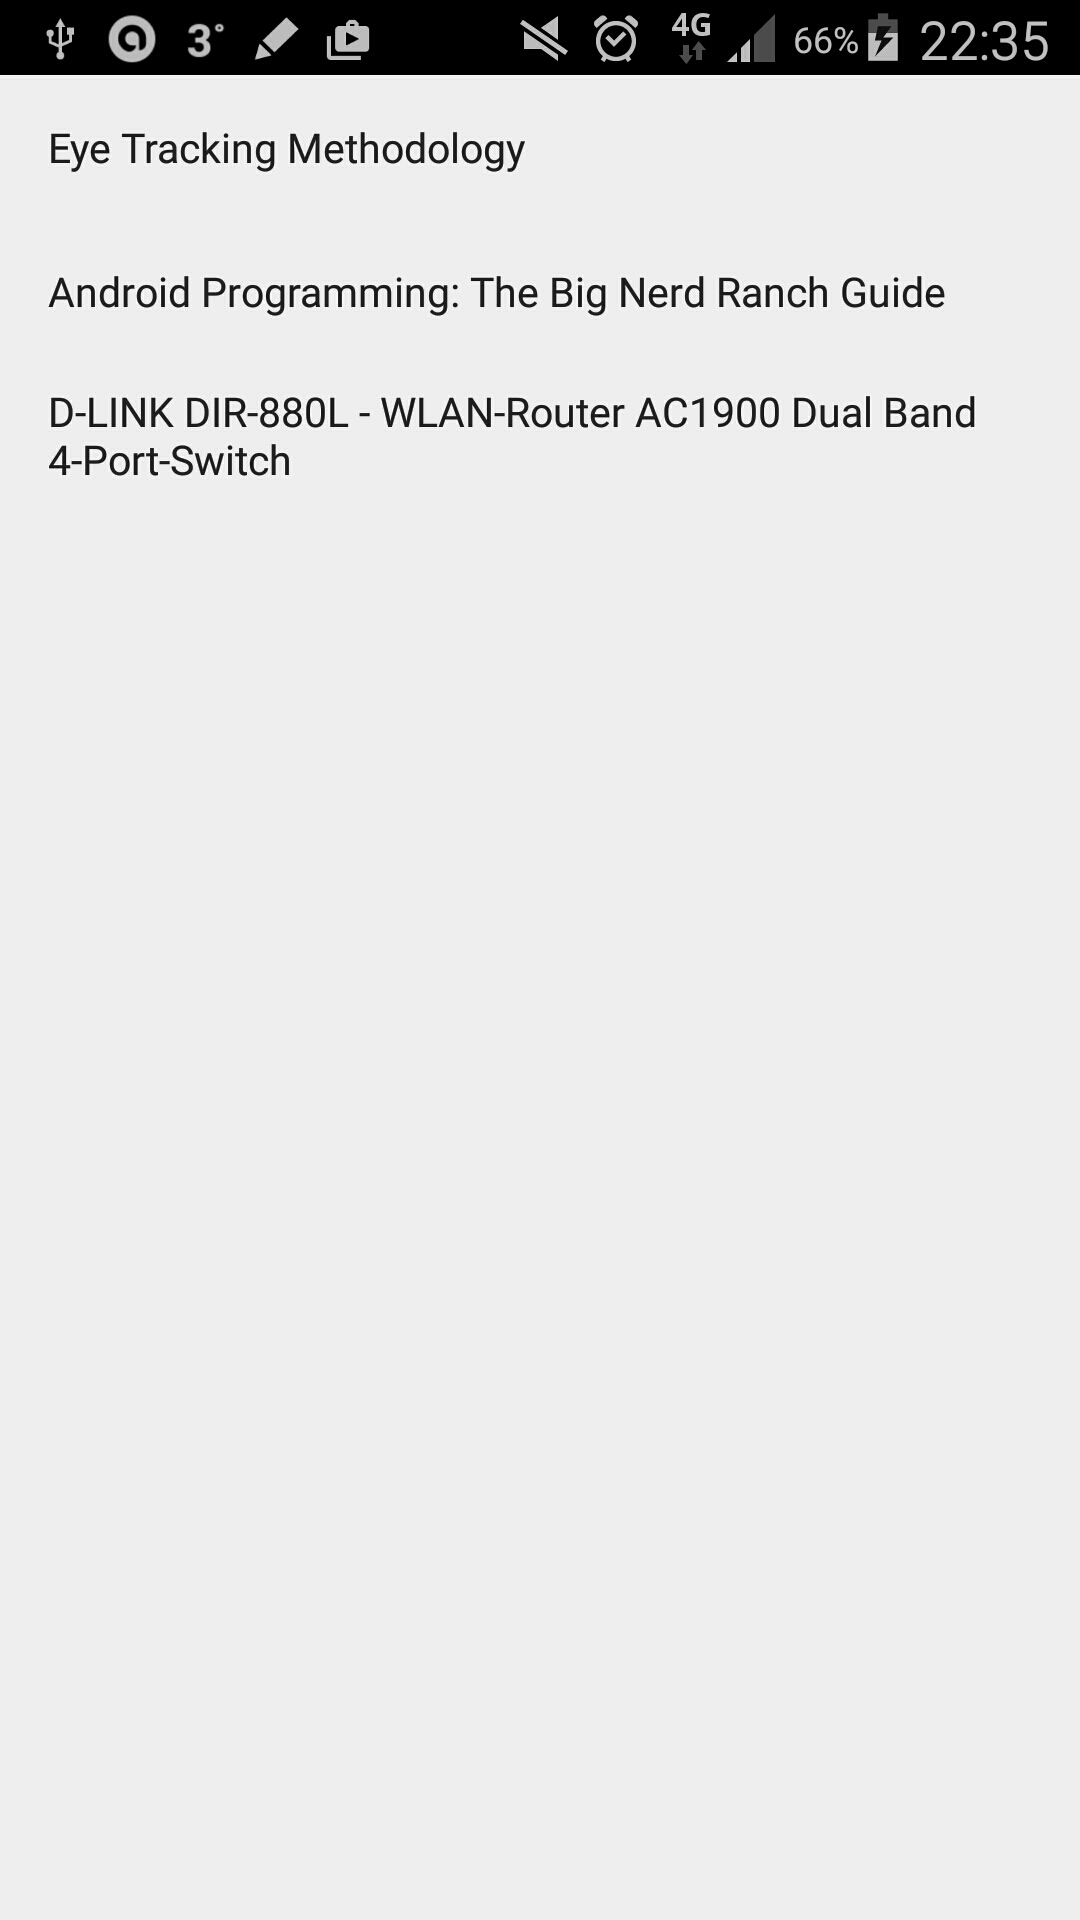
\includegraphics[width=0.9\linewidth]{List-Portrait.jpg}
		\caption{Portrait view of the List Activity.}
		\label{fig:list-view-portrait}
	\endminipage\hfill
\end{figure}

When running the Tingle App the first view the user sees is shown in Figure \ref{fig:tingle-view-portrait}. Since Version 4 (Mandatory Assignment \#1) not much has changed in the layout. The real changes in this version have been made under the hood. One main addition in the layout is the \emph{Scan Barcodes} button. If the user has a barcode scanner installed on their device they can scan a barcode for quick item-name lookup. The app uses Outpan to look up product information based on the barcode of the item. If no barcode scanner is installed on the device the \emph{Scan Barcode} button is changed to \emph{Lookup Barcode}, see Figure \ref{fig:lookupButton}, and the user can manually type in a barcode to fetch relevant product information. If the product the user is searching for exists on Outpan's servers then the name of the
product is added the \emph{What} field.

The rest of the features in this view are the same as in the previous version of the app. The user can add new things and their whereabouts to the database, search for exists things and finally list all things in the database. Clicking the button \texttt{List of All Things} will open up the List Activity shown in Figure \ref{fig:list-view-portrait}. The list view is a scrollable list showing all items in the database. Tapping an item in the list will toggle the \emph{What} (i.e the name of the item) and \emph{Where} (the location of the item). The user can also delete an item by Long pressing on an item.

\begin{figure}[!htb]
	\minipage{0.48\textwidth}
	\centering
	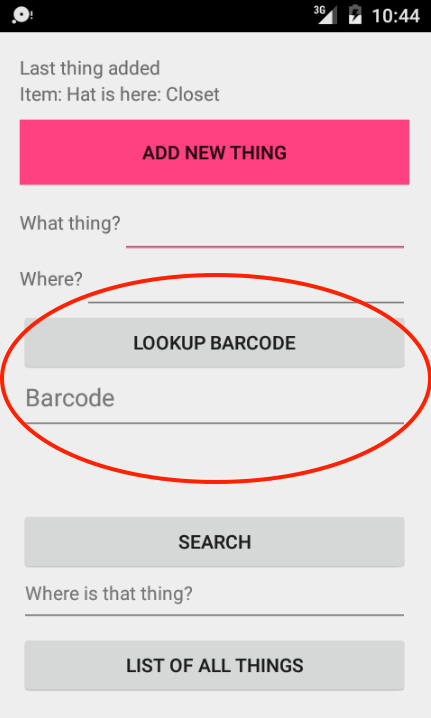
\includegraphics[width=0.9\textwidth]{BarcodeLookupButton.png}
	\caption{When no Barcode Scanner is found the user can still manually lookup product information.}
	\label{fig:lookupButton}
	\endminipage\hfill
	\minipage{0.48\textwidth}
	\centering
	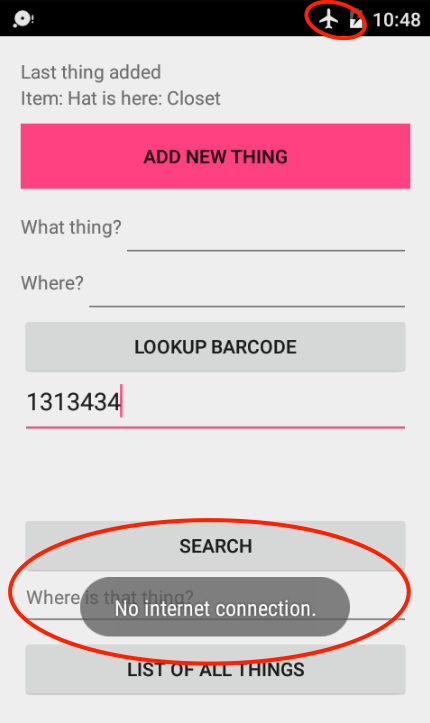
\includegraphics[width=0.9\textwidth]{NoInternet.png}
	\caption{If not internet connection is found the user is prompted with a Toast.}
	\label{fig:noInternet}
	\endminipage\hfill
\end{figure}

\pagebreak
Changing the orientation of the device to landscape displays the two views, \emph{Tingle view }and \emph{List view}, side-by-side. The same functionality applies to the views in landscape mode as they do in portrait mode as described above. The only difference is the removal of the \texttt{List of All Things} button since the list is already visible on the right side of the screen. This is a choice of design. One could also make it possible to open up the 
list in landscape view showing more information about each item.

\begin{figure}[H]
	\centering
	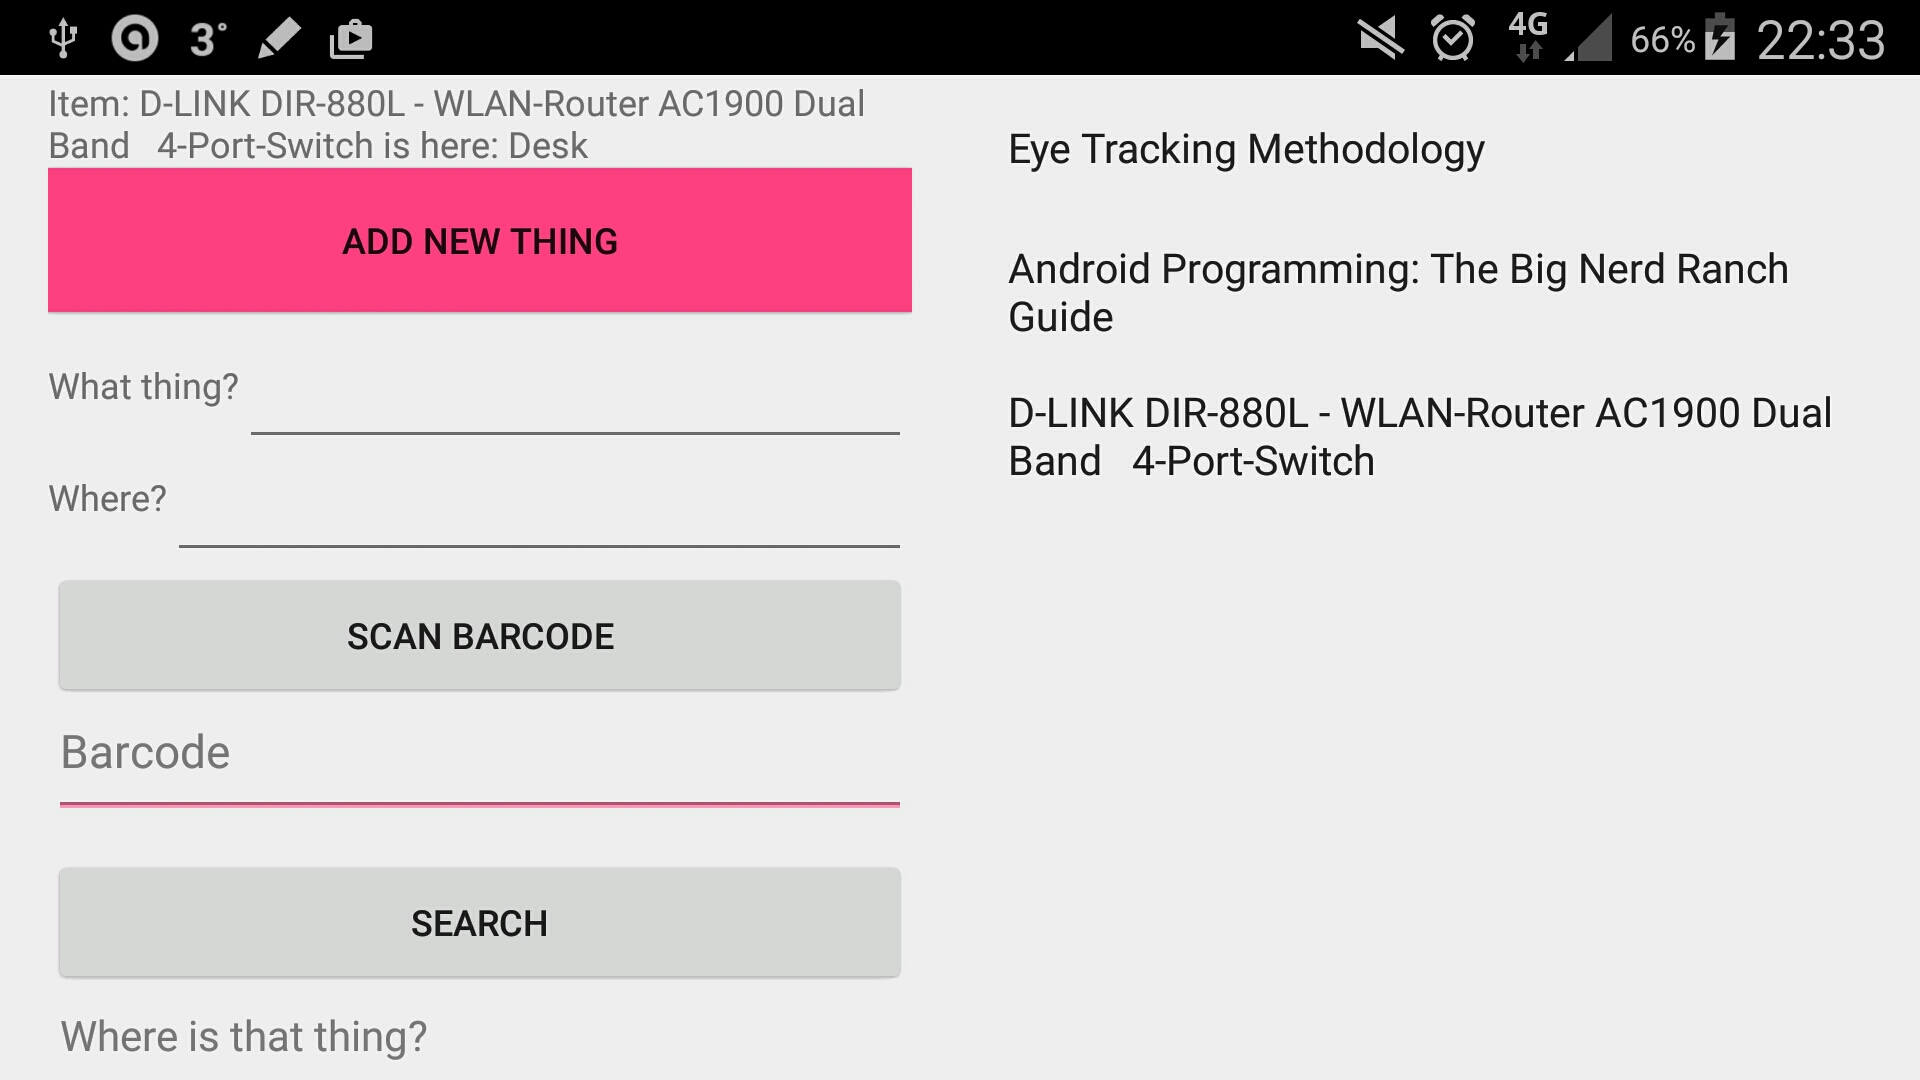
\includegraphics[width=0.7\textwidth]{Tingle-Dual.jpg}
	\caption{Landscape view showing both the main functions as well as the list of things side by side.}
	\label{fig:landscape-main-view}
\end{figure}

\section{Database}
Version 4 of Tingle App used an ArrayList to store data. The main issue with this implementation was that the data was not persistent. If the user closed the app all data was lost. This version of Tingle App uses an SQLite database to store data. The convention of the implementation of the SQLite database follows very closely chapter 14 in the book \emph{The Big Nerd Ranch Guide 2nd Edition}. With the SQLite database in store the data is now persistent even if the user closes the application.

\section{Search}
The user can search for items in the database using the \emph{Search} function in the main Tingle view. The search uses a simple SQL Query using the \texttt{"LIKE = "} clause to find items whose names contain the search query. If one or more results are returned only the first one is displayed to the user.

\section{Design}
\subsection{RecyclerView}
To be able to better handle if many items, say thousands, exist in the Tingle Database we use RecyclerViews. In the previous version of Tingle App every single item in the database were placed in their own TextView. Using a RecyclerView we circumvent this issue. Instead of creating a unique TextView for each item the RecyclerView only uses as many views as it takes to cover the whole screen plus a few more. When a view goes of the screen the view is reused with another item.

\section{Handling Missing Barcode Scanner}
If the device does not have a barcode scanner app installed the user can still manually lookup items using the given
barcode text field.

\section{Extensions }
Due to time constraints with other courses this version of the Tingle
App does not contain any extension over the minimum requirements.

\section{Testing}
The testing of the Tingle App has been separated into four different parts using only black-box testing. One for each view and one for each orientation of the device. As can been seen in the tables below the cases are similar for Portrait mode and Landscape mode. This redundant testing is done to make sure there are no unforeseen bugs when changing the orientation. When updated your application it is important to perform regression testing. Therefore many of the tests here are the same as in Mandatory Assignment \#1.

\begin{figure}[H]
	\centering
	\renewcommand*{\arraystretch}{1.5} % Redefine padding size
	\begin{tabular}{| c | p{3.5cm} | p{3.5cm} | p{3.5cm} |}
		\hline
		{\textbf{ID} } & {\textbf{Test Case} } & {\textbf{Expected Output}} & {\textbf {Actual Output}} \\\hline\hline
		% -- test 1
		A & Running the App & The application starts and the Tingle view is shown & The application starts and the Tingle view is shown  \\ \hline
		% -- test 2
		B &	Clicking the \texttt{List of All Things} button opens up the List view. & The List view is shown. & The List view is shown. \\ \hline
		C & It is possible to add an item to the database. & An item is successfully added to the database. & An item is successfully added to the database. \\ \hline
		D & It is possible to search for an item in the database. & A Toast is displayed showing the location of the found item. & A Toast is displayed showing the location of the found item. \\ \hline
		E & Clicking \texttt{List of All Things} opens up a the List view. 
     Clicking the android back button navigates back to the Tingle view & User is successfully navigated back to the Tingle view. & User is successfully navigated back to the Tingle view.  \\ \hline
     F & Click Scan Barcode when the device is online and try to scan a barcode. & A local Scanner Application opens and the user can scan for a barcode. If a product is found the name of the product is returned as well as the barcode itself. & If product is found the What field is filled with the name of the product. \\ \hline
     G & Click Scan Barcode when the device is offline. & A Toast appears notifying the user that the device is offline. & A Toast appears notifying the user that the device is offline. \\ \hline
     H & Type in a barcode and click Lookup Barcode when the device is online and no barcode scanner app exists on the device. & If a product is found the name of the product is returned to the What text field. & If product is found the What field is filled with the name of the product. \\ \hline
      I & Type in a barcode and click Lookup Barcode when the device is offline and no barcode scanner app exists on the device. & A Toast appears notifying the user that the device is offline. & A Toast appears notifying the user that the device is offline. \\ \hline
	\end{tabular}
	
	\caption{Test cases of the Tingle view in Portrait mode.}
	\label{tab:test-cases-tingle-portrait}
\end{figure}

\begin{figure}[H]
	\centering
	\renewcommand*{\arraystretch}{1.5} % Redefine padding size
	\begin{tabular}{| c | p{3.5cm} | p{3.5cm} | p{3.5cm} |}
		\hline
		{\textbf{ID} } & {\textbf{Test Case} } & {\textbf{Expected Output}} & {\textbf {Actual Output}} \\\hline\hline
		% -- test 1
		A & Running the App & Both the Tingle view and List view are shown side-by-side. & Both the Tingle view and List view are shown side-by-side.  \\ \hline
		% -- test 2
		B &	Clicking the \texttt{List of All Things} button in the Tingle view opens up the List view. & The List view is shown. & The List view is shown. \\ \hline
		C & It is possible to add an item to the database. & An item is successfully added to the database. & An item is successfully added to the database. \\ \hline
		D & It is possible to search for an item in the database. & A Toast is displayed showing the location of the found item. & A Toast is displayed showing the location of the found item. \\ \hline
		E & Changes in Layout compared to Portrait mode & The button \texttt{Lost of All Things} is not present. & The button \texttt{Lost of All Things} is not present. \\ \hline
	   F & Click Scan Barcode when the device is online and try to scan a barcode. & A local Scanner Application opens and the user can scan for a barcode. If a product is found the name of the product is returned as well as the barcode itself. & If product is found the What field is filled with the name of the product. \\ \hline
	   G & Click Scan Barcode when the device is offline. & A Toast appears notifying the user that the device is offline. & A Toast appears notifying the user that the device is offline. \\ \hline
	   H & Type in a barcode and click Lookup Barcode when the device is online and no barcode scanner app exists on the device. & If a product is found the name of the product is returned to the What text field. & If product is found the What field is filled with the name of the product. \\ \hline
	   I & Type in a barcode and click Lookup Barcode when the device is offline and no barcode scanner app exists on the device. & A Toast appears notifying the user that the device is offline. & A Toast appears notifying the user that the device is offline. \\ \hline
	\end{tabular}
	
	\caption{Test cases of the Tingle view in Landscape mode.}
	\label{tab:test-cases-tingle-landscape}
\end{figure}

\begin{figure}[H]
	\centering
	\renewcommand*{\arraystretch}{1.5} % Redefine padding size
	\begin{tabular}{| c | p{3.5cm} | p{3.5cm} | p{3.5cm} |}
		\hline
		{\textbf{ID} } & {\textbf{Test Case} } & {\textbf{Expected Output}} & {\textbf {Actual Output}} \\\hline\hline
		% -- test 1
		A &	It is possible to click an item in the list & Toggles Name / Location of the item.  & Toggles Name / Location of the item. \\ \hline
		B & It is possible to Long click an item in the list. & A dialog is displayed asking if the user wants to delete the clicked item. & A dialog is displayed asking if the user wants to delete the clicked item. \\ \hline
		C & When deleting an item the user can decline the request by pressing \texttt{No}. & The item is not deleted. & The item is not deleted. \\ \hline
		D & When deleting an item the user can accept the request by pressing \texttt{Yes}. & The item is deleted from the list. & The item is deleted from the list. \\ \hline
		E & It is possible to delete items one by one until the list is empty. & All items are deleted and the app does not crash. & All items are deleted and the app does not crash. \\ \hline
		F & If there are many items in the database and not all items fit on the screen the user
		can scroll the list. & The list is scrollable. & The list is scrollable. \\ \hline
	\end{tabular}
	
	\caption{Test cases of the List view in Portrait mode.}
	\label{tab:test-cases-list-portrait}
\end{figure}

\begin{figure}[H]
	\centering
	\renewcommand*{\arraystretch}{1.5} % Redefine padding size
	\begin{tabular}{| c | p{3.5cm} | p{3.5cm} | p{3.5cm} |}
		\hline
		{\textbf{ID} } & {\textbf{Test Case} } & {\textbf{Expected Output}} & {\textbf {Actual Output}} \\\hline\hline
		% -- test 1
		A &	It is possible to click an item in the list & Toggles Name / Location of the item.  & Toggles Name / Location of the item. \\ \hline
		B & It is possible to Long click an item in the list. & A dialog is displayed asking if the user wants to delete the clicked item. & A dialog is displayed asking if the user wants to delete the clicked item. \\ \hline
		C & When deleting an item the user can decline the request by pressing \texttt{No}. & The item is not deleted. & The item is not deleted. \\ \hline
		D & When deleting an item the user can accept the request by pressing \texttt{Yes}. & The item is deleted from the list. & The item is deleted from the list. \\ \hline
		E & It is possible to delete all items in the list. & All items are deleted. & All items are deleted. \\ \hline
		F & If there are many items in the database and not all items fit on the screen the user can scroll the list. & The list is scrollable. & The list is scrollable. \\ \hline
	\end{tabular}
	
	\caption{Test cases of the List view in Landscape mode.}
	\label{tab:test-cases-list-landscape}
\end{figure}